% -*- latex -*-
%%%%%%%%%%%%%%%%%%%%%%%%%%%%%%%%%%%%%%%%%%%%%%%%%%%%%%%%%%%%%%%%
%%%%%%%%%%%%%%%%%%%%%%%%%%%%%%%%%%%%%%%%%%%%%%%%%%%%%%%%%%%%%%%%
%%%%
%%%% This text file is part of the source of 
%%%% `Introduction to High-Performance Scientific Computing'
%%%% by Victor Eijkhout, copyright 2012-7
%%%%
%%%% This book is distributed under a Creative Commons Attribution 3.0
%%%% Unported (CC BY 3.0) license and made possible by funding from
%%%% The Saylor Foundation \url{http://www.saylor.org}.
%%%%
%%%%
%%%%%%%%%%%%%%%%%%%%%%%%%%%%%%%%%%%%%%%%%%%%%%%%%%%%%%%%%%%%%%%%
%%%%%%%%%%%%%%%%%%%%%%%%%%%%%%%%%%%%%%%%%%%%%%%%%%%%%%%%%%%%%%%%

\index{red-black ordering|(}
\index{matrix ordering!red-black dissection|see{red-black ordering}}

Another permutation of the problem variables is based on graph colouring
(section~\ref{sec:independent}). The direct goal here is to maximize
available parallelism.

Let us take a
simple example, where $A$ is a tridiagonal matrix. The equation $Ax=b$
looks like
\[ 
\begin{pmatrix}
  a_{11}&a_{12}&&&&\emptyset\\ a_{21}&a_{22}&a_{23}\\ 
  &a_{32}&a_{33}&a_{34}\\ \emptyset&&\ddots&\ddots&\ddots
\end{pmatrix}
\begin{pmatrix}  x_1\\ x_2\\ x_3\\ \vdots\end{pmatrix} =
\begin{pmatrix}  y_1\\ y_2\\ y_3\\ \vdots\end{pmatrix}
\]
We observe that $x_i$ directly depends on $x_{i-1}$ and~$x_{i+1}$, but
not $x_{i-2}$ or~$x_{i+1}$. Thus, let us see what happens if we
permute the indices to group every other component together.

Pictorially, we take the points $1,\ldots,n$ and colour them red and
black (figure~\ref{fig:red-black-1d}), then we permute them to first
\begin{figure}
  \begin{quote}
    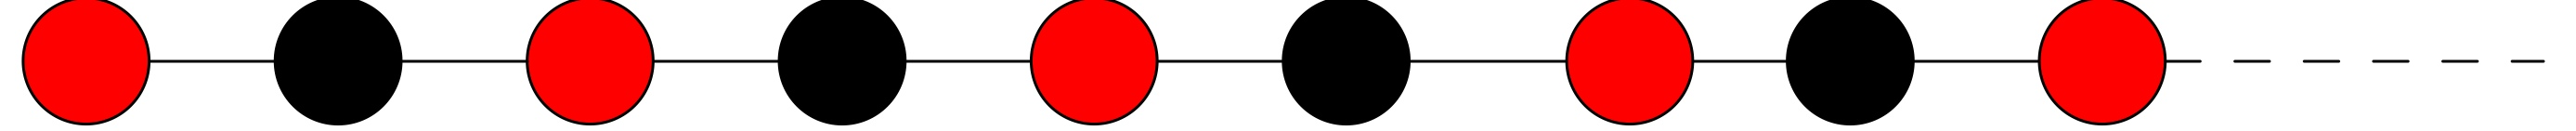
\includegraphics[scale=.12]{graphics/red-black-1d}
  \end{quote}
  \caption{Red-black ordering of a the points on a line}
  \label{fig:red-black-1d}
\end{figure}
take all red points, and subsequently all black ones.
The correspondingly permuted matrix looks as follows:
\[ 
\begin{pmatrix}
  a_{11}&&&&a_{12}\\ &a_{33}&&&a_{32}&a_{34}\\ &&a_{55}&&&\ddots&\ddots\\
  &&&\ddots\\
  a_{21}&a_{23}&&&a_{22}\\ &a_{43}&a_{45}&&&a_{44}\\ &&\ddots&\ddots&&&\ddots
\end{pmatrix}
\begin{pmatrix}  x_1\\ x_3\\ x_5\\ \vdots\\ x_2\\ x_4\\ \vdots\end{pmatrix} =
\begin{pmatrix}  y_1\\ y_3\\ y_5\\ \vdots\\ y_2\\ y_4\\ \vdots\end{pmatrix}
\]
With this permuted $A$, the Gauss-Seidel matrix $D_A+L_A$ looks like
\[ 
\begin{pmatrix}
  a_{11}&&&&\emptyset\\ &a_{33}\\ &&a_{55}\\
  &&&\ddots\\
  a_{21}&a_{23}&&&a_{22}\\ &a_{43}&a_{45}&&&a_{44}\\ &&\ddots&\ddots&&&\ddots
\end{pmatrix}
\]
What does this buy us? Well, let's spell out the solution of a system
$Lx=y$.

\begin{displayalgorithm}
  \For{$i=1,3,5,\ldots$}{solve $x_i\leftarrow y_i/a_{ii}$}
  \For{$i=2,4,6,\ldots$}{compute $t=a_{ii-1}x_{i-1}+a_{ii+1}x_{i+1}$
    \; solve $x_i\leftarrow (y_i-t)/a_{ii}$
  }
\end{displayalgorithm}

Apparently the algorithm has three stages that are each parallel over
half the domain points. This is illustrated in
figure~\ref{fig:1d-rb-solve}.
\begin{figure}[ht]
  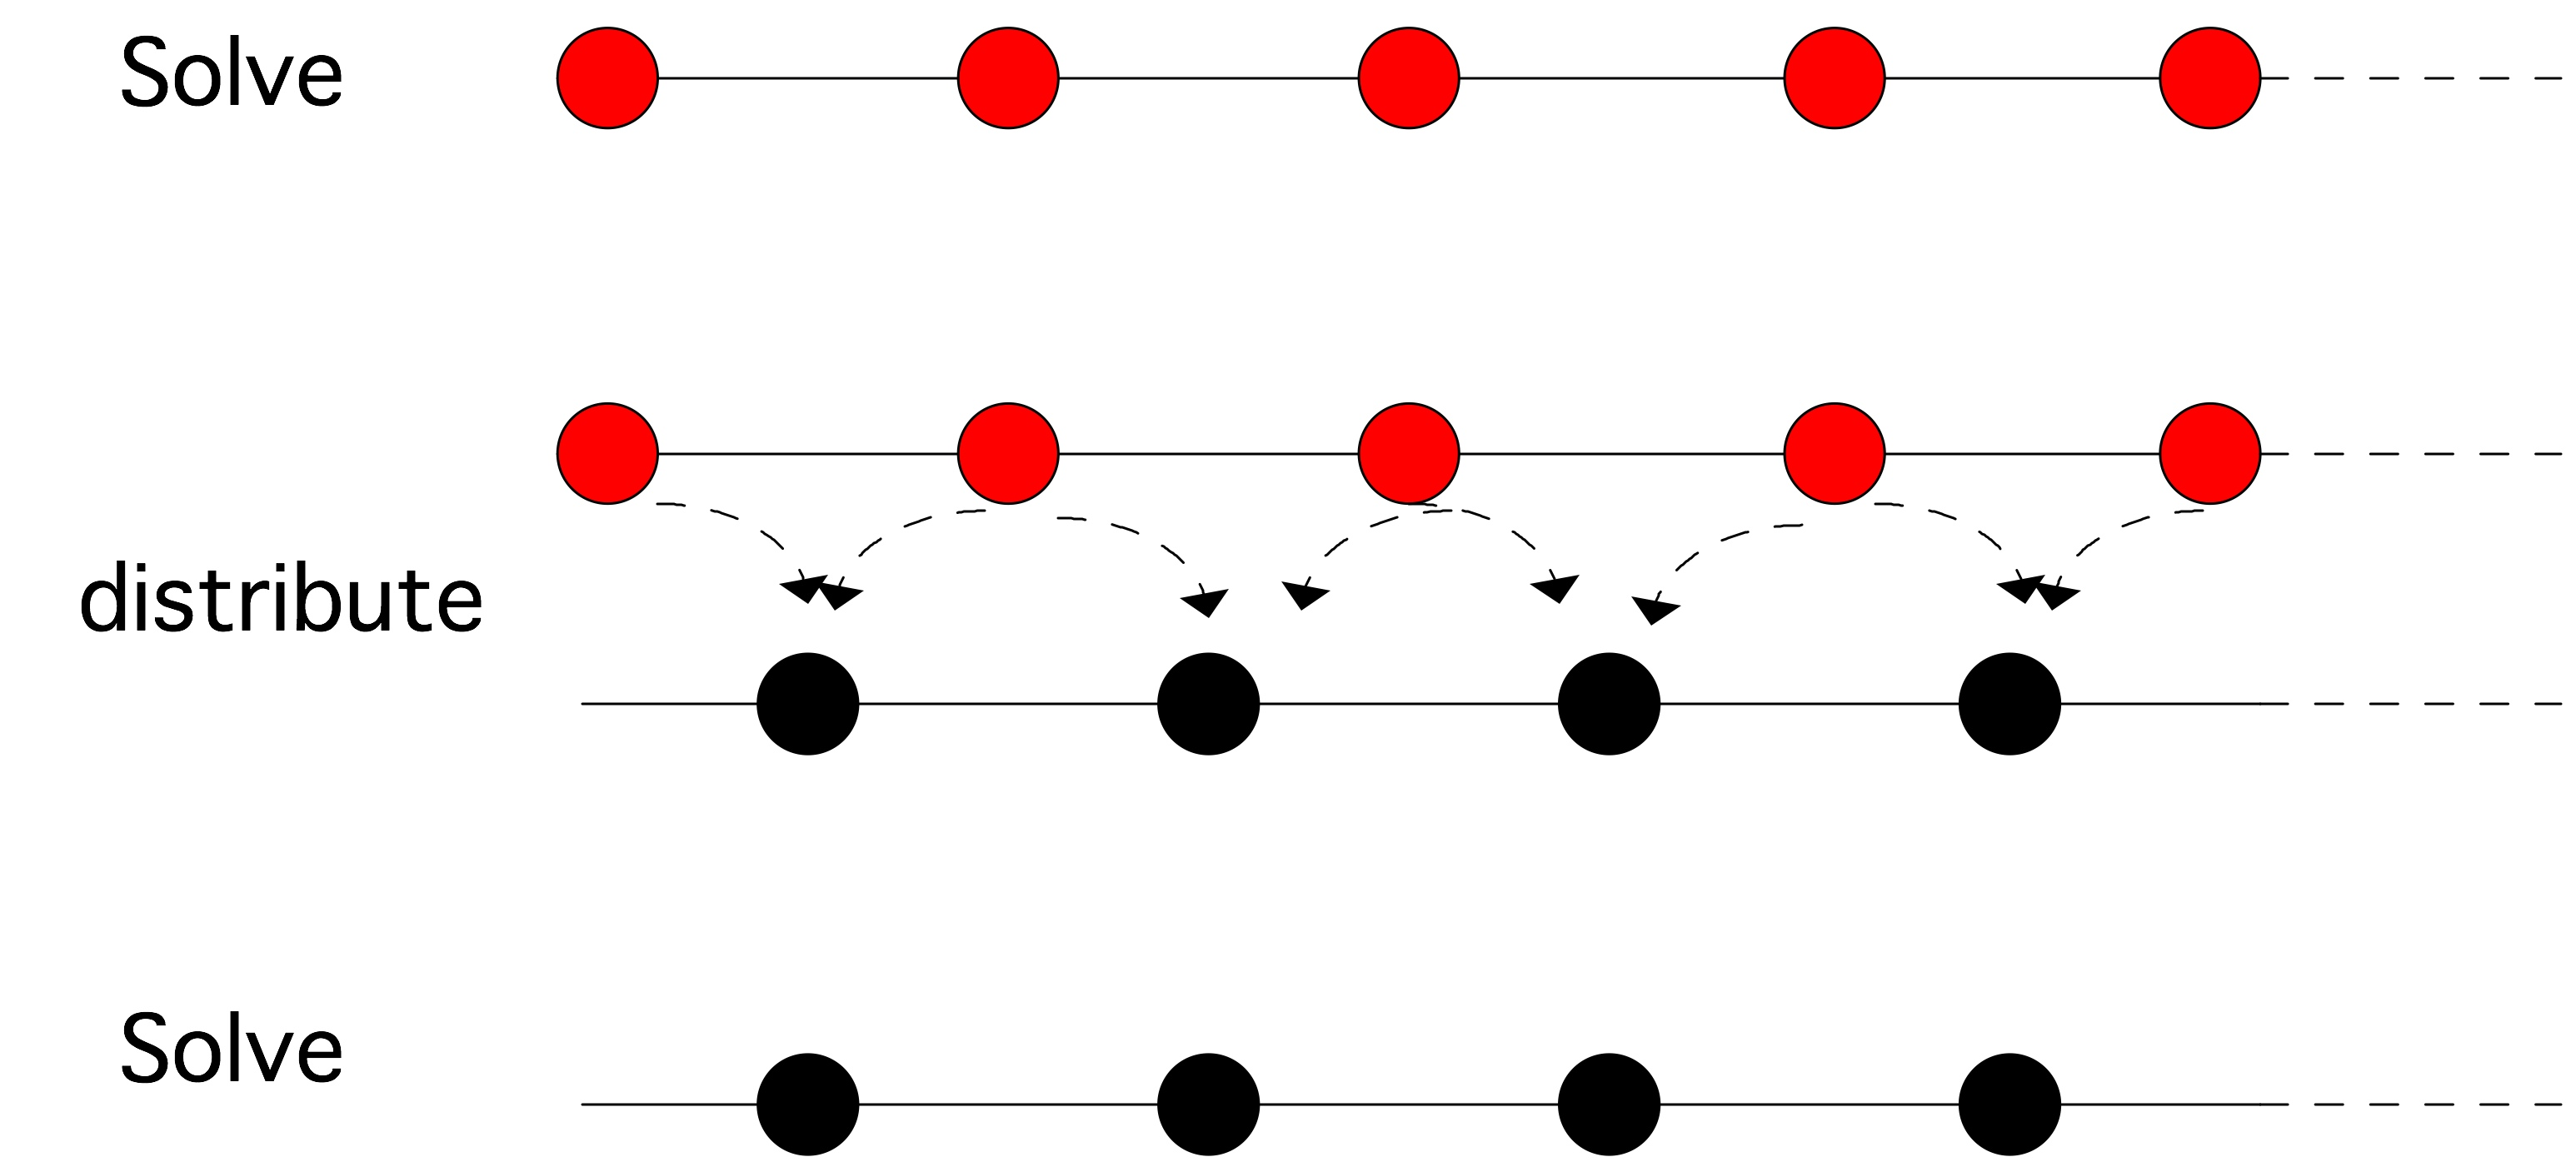
\includegraphics[scale=.1]{graphics/red-black-1d-solve}
  \caption{Red-black solution on a 1d domain}
  \label{fig:1d-rb-solve}
\end{figure}
Theoretically we could accommodate a number of processors that is half
the number of the domain points, but in practice each processor will
have a subdomain. Now you can see in figure~\ref{fig:1d-rb-solve-par}
how this causes a very modest amount of communication: each processor
sends at most the data of two red points to its neighbours.
\begin{figure}[ht]
  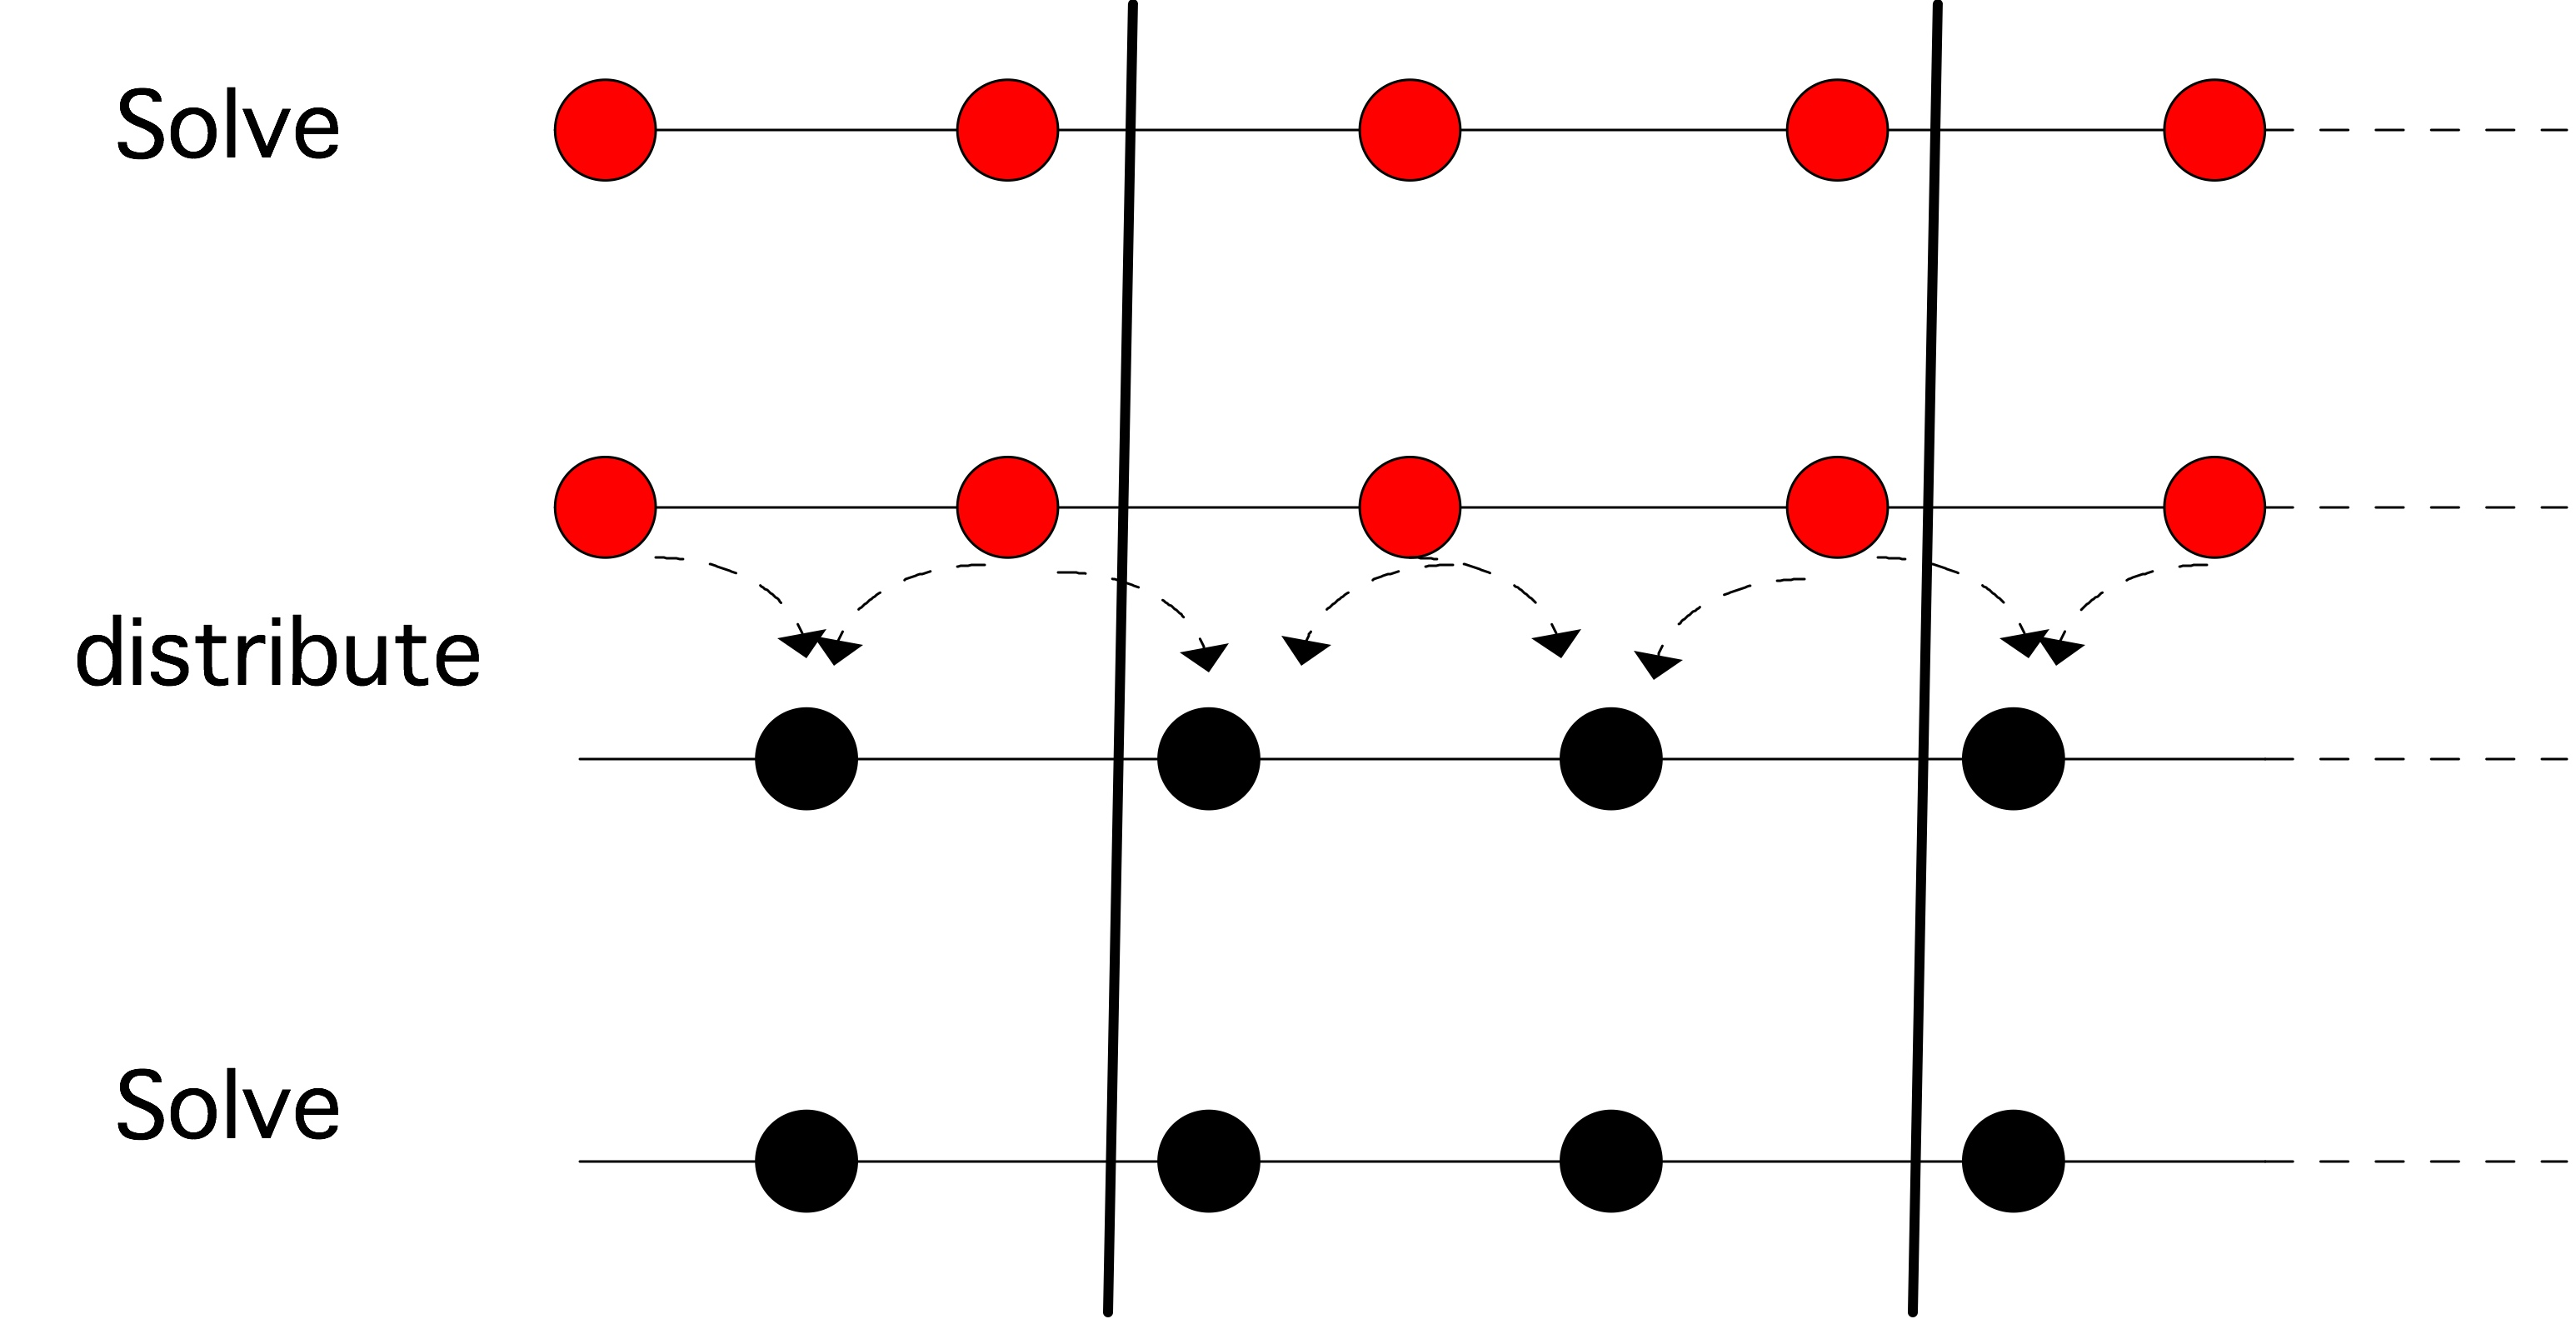
\includegraphics[scale=.1]{graphics/red-black-1d-solve-par}
  \caption{Parallel red-black solution on a 1d domain}
  \label{fig:1d-rb-solve-par}
\end{figure}

Red-black ordering can be applied to two-dimensional problems too.
Let us apply a red-black ordering to the points $(i,j)$ where $1\leq
i,j\leq n$.
Here we first apply a successive numbering to the odd
points on the first line $(1,1),(3,1),(5,1),\ldots$, then the even
points of the second line $(2,2),(4,2),(6,2),\ldots$, the odd points
on the third line, et cetera. Having thus numbered half the points in
the domain, we continue with the even points in the first line, the
odd points in the second, et cetera.
\begin{figure}[ht]
  \begin{quote}
    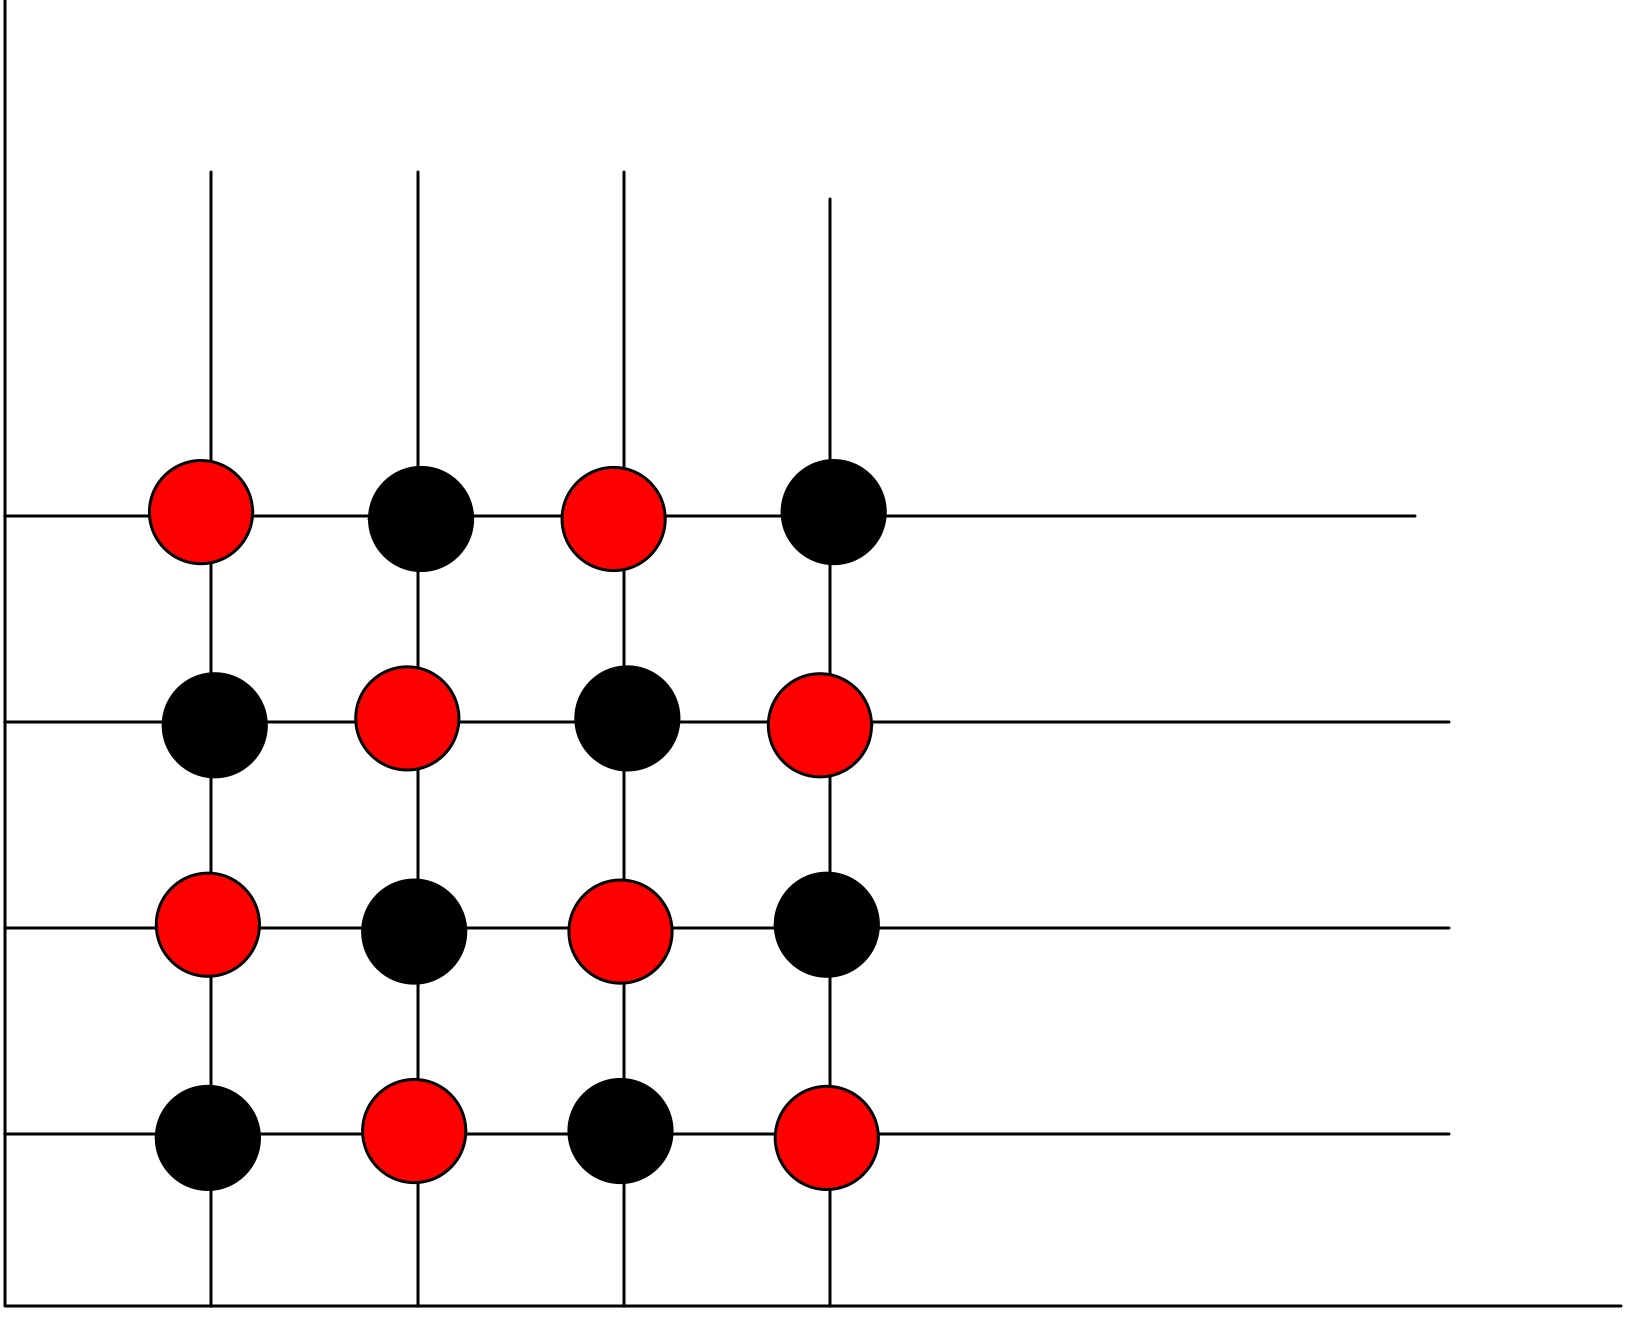
\includegraphics[scale=.12]{graphics/redblack}
  \end{quote}
  \caption{Red-black ordering of the variables of a two-dimensional
    domain}
  \label{fig:redblack}
\end{figure}
As you can see in figure~\ref{fig:redblack}, now the red points are
only connected to black points, and the other way around. In graph
theoretical terms, you have found a \indexterm{colouring} 
(see appendix~\ref{app:graph} for the definition
of this concept) of the matrix graph with two colours.

\begin{exercise}
  Apply the red-black ordering to the 2D \ac{BVP} \eqref{eq:laplace}.
  Sketch the resulting matrix structure.
\end{exercise}

The red-black ordering is a simple
example of \indextermbus{graph}{colouring} (sometimes called
\indexterm{multi-colouring}). In
simple cases, such as the unit square domain we considered in
section~\ref{sec:2dbvp} or its extension to 3D, the \indexterm{colour
  number} of the adjacency graph is easily determined.

\begin{exercise}
  You saw that a red-black ordering of unknowns
  coupled with the regular five-point star stencil give two subsets of
  variables that are not connected among themselves, that is, 
  they form a two-colouring of the matrix graph. 
  Can you find a colouring if nodes are connected by the second stencil in
  figure~\ref{fig:stencils}?
\end{exercise}

\index{red-black ordering|)}

There is a simple bound for the number of colours needed for the graph
of a sparse matrix: the number of colours is at most $d+1$ where
$d$~is the degree of the graph. To see that we can colour a graph with
degree~$d$ using $d+1$ colours, consider a node with
degree~$d$. No matter how its neighbours are coloured, there is always
an unused colour among the $d+1$ available ones.

\begin{exercise}
  Consider a sparse matrix, where the graph can be coloured with $d$
  colours. Permute the matrix by first enumerating the unknowns of the
  first colour,
  then the second colour, et cetera. What can you say about the
  sparsity pattern of the resulting permuted matrix?
\end{exercise}

If you
are looking for a direct solution of the linear system you can repeat
the process of colouring and permuting on the matrix that remains
after you have eliminated one colour. In the case of a tridiagonal
matrix you saw that this remaining matrix was again tridiagonal, so
it is clear how to continue the process. This is called
\indexterm{recursive doubling}. If the matrix is not tridiagonal but
\indexterm{block tridiagonal}, this operation can be performed on
blocks.

